\documentclass{standalone}

\usepackage{tikz}
\usepackage{bm}

\usetikzlibrary{patterns}
\usetikzlibrary{arrows.meta}

\usetikzlibrary{decorations.pathreplacing, decorations.markings}
\tikzset{
    midarrow/.style={
        decoration={markings, mark=at position 0.33 with {\arrow{Latex}}},
        postaction={decorate}
    }
}

\begin{document}

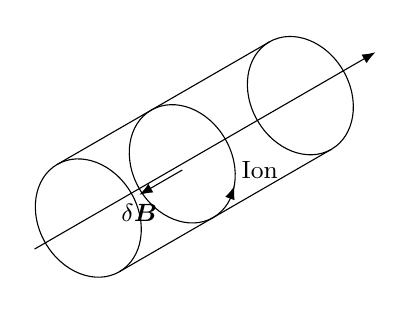
\begin{tikzpicture}

	\def\angle{30}
	\def\length{5}
	\def\radiusx{0.63}
	\def\radiusy{\radiusx*1.25}	
	
	\pgfmathsetmacro{\xend}{cos(\angle)*\length};
	\pgfmathsetmacro{\yend}{sin(\angle)*\length};
	
	\draw[ -{Latex} ] (0, 0) -- (\xend, \yend);
	
	\draw[ rotate=\angle ] (\radiusy, 0) ellipse (\radiusx cm and \radiusy cm);
	
	\draw[ rotate=\angle ] (\xend*0.9, 0) ellipse (\radiusx cm and \radiusy cm);
	
	\draw[ rotate=\angle ] (\xend*0.5, 0) ellipse (\radiusx cm and \radiusy cm);
	\draw[ -{Latex}, rotate=\angle ] (\xend*0.585
	,-\radiusy*0.8) -- (\xend*0.6,-\radiusy*0.73);
	
	\draw[ rotate=\angle ] (\radiusy, -\radiusy) -- (\xend*0.9, -\radiusy);
	\draw[ rotate=\angle ] (\radiusy, \radiusy) -- (\xend*0.9, \radiusy);
	
	\pgfmathsetmacro{\xmid}{\xend*0.5*cos(\angle)}
	\pgfmathsetmacro{\ymid}{\xend*0.5*sin(\angle)-\radiusy/10}
	\pgfmathsetmacro{\xflec}{(\xend*0.5-\radiusx)*cos(\angle)}
	\pgfmathsetmacro{\yflec}{(\xend*0.5-\radiusx)*sin(\angle)-\radiusy/10}
		
	\draw[ -{Latex} ] (\xmid, \ymid) -- (\xflec, \yflec) node[ anchor=north ] {\small \( \delta \bm{B} \)};
	
	\node[ anchor=west ] at (\xmid+\radiusx, \ymid) {\small Ion};

\end{tikzpicture}

\end{document}